Heterogeneous catalysis, electrochemical energy conversion, and surface-mediated synthesis depend critically on identifying the most stable adsorbate--surface configurations.
The configuration space for this problem grows combinatorially: site types (ontop, bridge, hollow, and their compositional variants), adsorbate orientation, and conformational flexibility combine to produce candidate counts exceeding several hundred for a single intermetallic surface with a polyatomic adsorbate.
Traditional approaches---DFT enumeration, genetic algorithms, basin hopping---require many energy evaluations, each costing hundreds to thousands of CPU-hours, and scale poorly to the complex alloy and multimetallic surfaces of greatest practical interest.

% the related paradigms are divided into 2 parts: MLFF and LLM
%% they reflect some existing shortage, but I think should be organized in this logic: 
%%% MLFF, MLFF work and limitations; LLM, LLM work and limitations; their combined work like CatDT?
\subsection{Machine learning surrogates and the remaining search problem}
With the development of deep learning, Machine learning force fields (MLFFs) such as MACE/MACE-MP~\cite{batatia2022mace,batatia2023foundation}, CHGNet~\cite{deng2023chgnet}, and Equiformer~\cite{liao2023equiformerv2} have dramatically reduced the per-evaluation cost, achieving near-DFT accuracy at orders-of-magnitude speedup.
However, MLFFs solve only the \textit{fast energy evaluation} problem; they do not address the upstream \textit{search strategy} problem of deciding which configurations to evaluate.
Deep-learning-assisted configuration generators---graph neural networks that predict site stability, diffusion models that propose structures---remain open-loop: once trained, they cannot adapt based on new calculation results.
This architectural limitation causes systematic failures on surfaces where training-data coverage is sparse, precisely the complex compositions where better search is most needed.

% this part needs to be thought where to move, just for reference? maybe the end of intro
\textit{Adsorption configuration search.}
Classical approaches include exhaustive DFT enumeration on canonical site families, genetic algorithms~\cite{vilhelmsen2014genetic}, basin hopping~\cite{wales1997global}, and random structure search~\cite{pickard2011ab}.
More recent work uses MLFFs as fast evaluators inside these loops, including AdsorbML on the Open Catalyst 2020 Dense benchmark~\cite{lan2023adsorbml} and heuristic enumerators such as Autoadsorbate~\cite{fako2025simple}.
These methods are reliable (brute force does not fail silently) but scale linearly with configuration-space size; our results confirm that they reach lower energies than AdsMind on complex surfaces, at the cost of 5--25$\times$ more relaxations.


\subsection{LLM agents: capability and reliability gaps}
At the same time, the emergence of Large Language Model (LLM) agents have raised a promiising strategy of search problem, with their encoded scientific intuition from their vast training corpora.
Existing works have combined the strengths of fast physical simulation and LLM agent for  scientific results search and evaluation. 
% not sure to put the related agentic framework here, but they need a simple intro
% 我们目前家的内容不太对感觉，catdt可能会在这个论文之后挂出来，不然这个很难投稿呀，所以不要include哦

% if we introduce them here, it should become kind of a background of LLM agents
For example, CatDT...
Simpoly...
Scalable Machine Learning Force Field...
Autonomous Quantum Simulation through Large Language Model Agents...
%这些是我们自己的工作，并不是相关工作。


For adsorption config search, Adsorb-Agent was designed with a single-pass LLM planner and EquiformerV2, which enables it to generate plausible adsorption hypotheses from natural-language surface descriptions and execute fast physical simulation.
Related efforts include ChemCrow~\cite{bran2024chemcrow} (tool-augmented LLM for synthesis planning), Coscientist~\cite{boiko2023autonomous} (autonomous chemistry experimentation), and early closed-loop retrosynthesis agents~\cite{schwaller2020predicting}.

% main comparison, we need to point out the uniqueness of adsorb-agent among these architectures
Adsorb-Agent~\cite{ock2024adsorbagent} demonstrated that an LLM agent can propose initial site selections and enumerate configurations at each, reducing the effective search space relative to naive DFT sweeps.

However, existing LLM agents operate in a \textit{single-pass} regime: the LLM proposes configurations, relaxations execute, the lowest-energy result is reported, and the LLM is never informed of the physical outcome.
This architectural choice has two consequences we quantify in this work.
First, \textit{reliability suffers:} when the LLM's initial site prediction does not match any geometrically enumerable site on the surface, the system produces zero valid configurations and fails silently. We observe this failure mode on 20--27\% of cases across GPT-4o and GPT-5.4, with failure patterns that differ between LLMs, indicating an irreducible architectural limit rather than a model-capability artifact.
Second, \textit{interpretability suffers:} the system cannot distinguish a thermodynamically unstable site from a simulation failure, cannot learn from dissociation or rearrangement events, and cannot correct the systematic biases all current LLMs carry---preferring high-symmetry sites, underweighting surface composition effects, and ignoring adsorbate conformational flexibility.
% None have been evaluated head-to-head against non-LLM baselines \textit{under identical MACE-MP-0 small physics}, leaving open whether reported gains reflect planning quality or force-field/backbone choice.


%% why we need to introduce the benchmarks here??
% \textit{LLM evaluation in scientific domains.}
% Benchmarks such as ChemBench~\cite{mirza2024chembench}, MatBench~\cite{dunn2020benchmarking}, and SciEval~\cite{sun2024scieval} test factual recall and text-based reasoning but not applied chemical prediction.
% Chemical Slip, introduced in this work, is a physically grounded complementary signal: it quantifies whether an LLM's structural hypothesis survives physical relaxation, measured automatically from relaxation trajectories.



\subsection{Closing the loop: reliability, efficiency, and interpretability}
% this section introduces the key idea of AdsMind
To overcome the weakness of single-pass reasoning and feedback the physical information, We introduce AdsMind, a closed-loop multi-agent framework in which each MLFF relaxation result feeds back into the LLM planner, enabling the system to detect its own reasoning errors, encode them as actionable search constraints, and decide autonomously when to stop.
Three mechanisms implement this feedback cycle:

\begin{enumerate}
    \item \textbf{Chemical Slip detection.} After each relaxation, the analyzer compares the planner's intended adsorption site with the realized coordination environment. A mismatch---termed a \textit{Chemical Slip}---signals that the potential energy surface (PES) topology disagrees with the LLM's chemical intuition at that point, providing a physically grounded diagnostic of planner error.
    \item \textbf{FORBID constraints.} Detected slips and dissociation events are converted into explicit negative constraints in the planner's prompt history, preventing the agent from retrying site families that have already proven unstable or misclassified.
    \item \textbf{Autonomous termination.} The agent monitors whether successive iterations converge to the same best energy and terminates early when further exploration is unlikely to improve the result.
\end{enumerate}

We frame this design through a sequential-decision lens: adsorption configuration search is analogous to a partially observable Markov decision process (POMDP), where the PES is the hidden state, each relaxation is an observation, and the planner's next proposal is conditioned on the full history of prior observations.
Open-loop methods use a fixed policy $\pi(a \mid s)$ that cannot adapt after deployment; AdsMind approximates a history-dependent policy $\pi(a \mid h_t)$ through the LLM's in-context learning, without explicit reward engineering or policy optimization.

On the currently complete evaluation tracks, this closed-loop design yields a consistent reliability advantage across chemically broader surfaces.
On CMU20, AdsMind Full succeeds on 80/80 runs across four backends while the 1-Shot control drops to 73/80.
On the expanded OCD24 benchmark, the four-backend clean matrix gives 96/96 Full successes versus 82/96 for 1-Shot.
On the broader 50-case OCD rep50 slice, the same four-backend comparison gives 197/200 Full successes versus 178/200 for 1-Shot.
These completed tracks already indicate that the main value of closing the loop is not deeper basin discovery, but a reproducible gain in reliability and backend robustness across surfaces where open-loop planning is brittle.


\textit{Our contribution in this landscape.}
We believe this is the first study to (i)~run four distinct LLM backends on an identical closed-loop search pipeline, (ii)~compare an LLM agent head-to-head against non-LLM baselines (random, heuristic) and an LLM baseline (Adsorb-Agent) under \textit{matched} MACE-MP-0 physics, and (iii)~report explicit negative results on energy-depth to clarify the operating envelope in which closed-loop LLM reasoning adds value.

We also report, as negative results, that AdsMind does not deliver the deepest energy basins on complex surfaces: broader initial sampling strategies consistently reach lower minima when they succeed.
This trade-off---reliability and efficiency against depth of exploration---frames the central message of the paper.
AdsMind is not a replacement for brute-force methods where compute is cheap and failures are tolerable; it is a foundation for \textit{autonomous chemistry workflows} where silent failures, irreproducibility, and uninterpretable failures are unacceptable, and where compute is expensive enough that a 5--25$\times$ efficiency gain matters.
A natural extension, outlined in the Conclusion, couples AdsMind's closed-loop error recovery with broader initial site enumeration to combine the reliability of the former with the depth of the latter.

Head-to-head comparisons against Adsorb-Agent were performed by forking the original codebase and replacing its EquiformerV2 backend with the same MACE-MP-0 small calculator used in the primary benchmark, ensuring apples-to-apples physics.

\begin{figure}
    \centering
    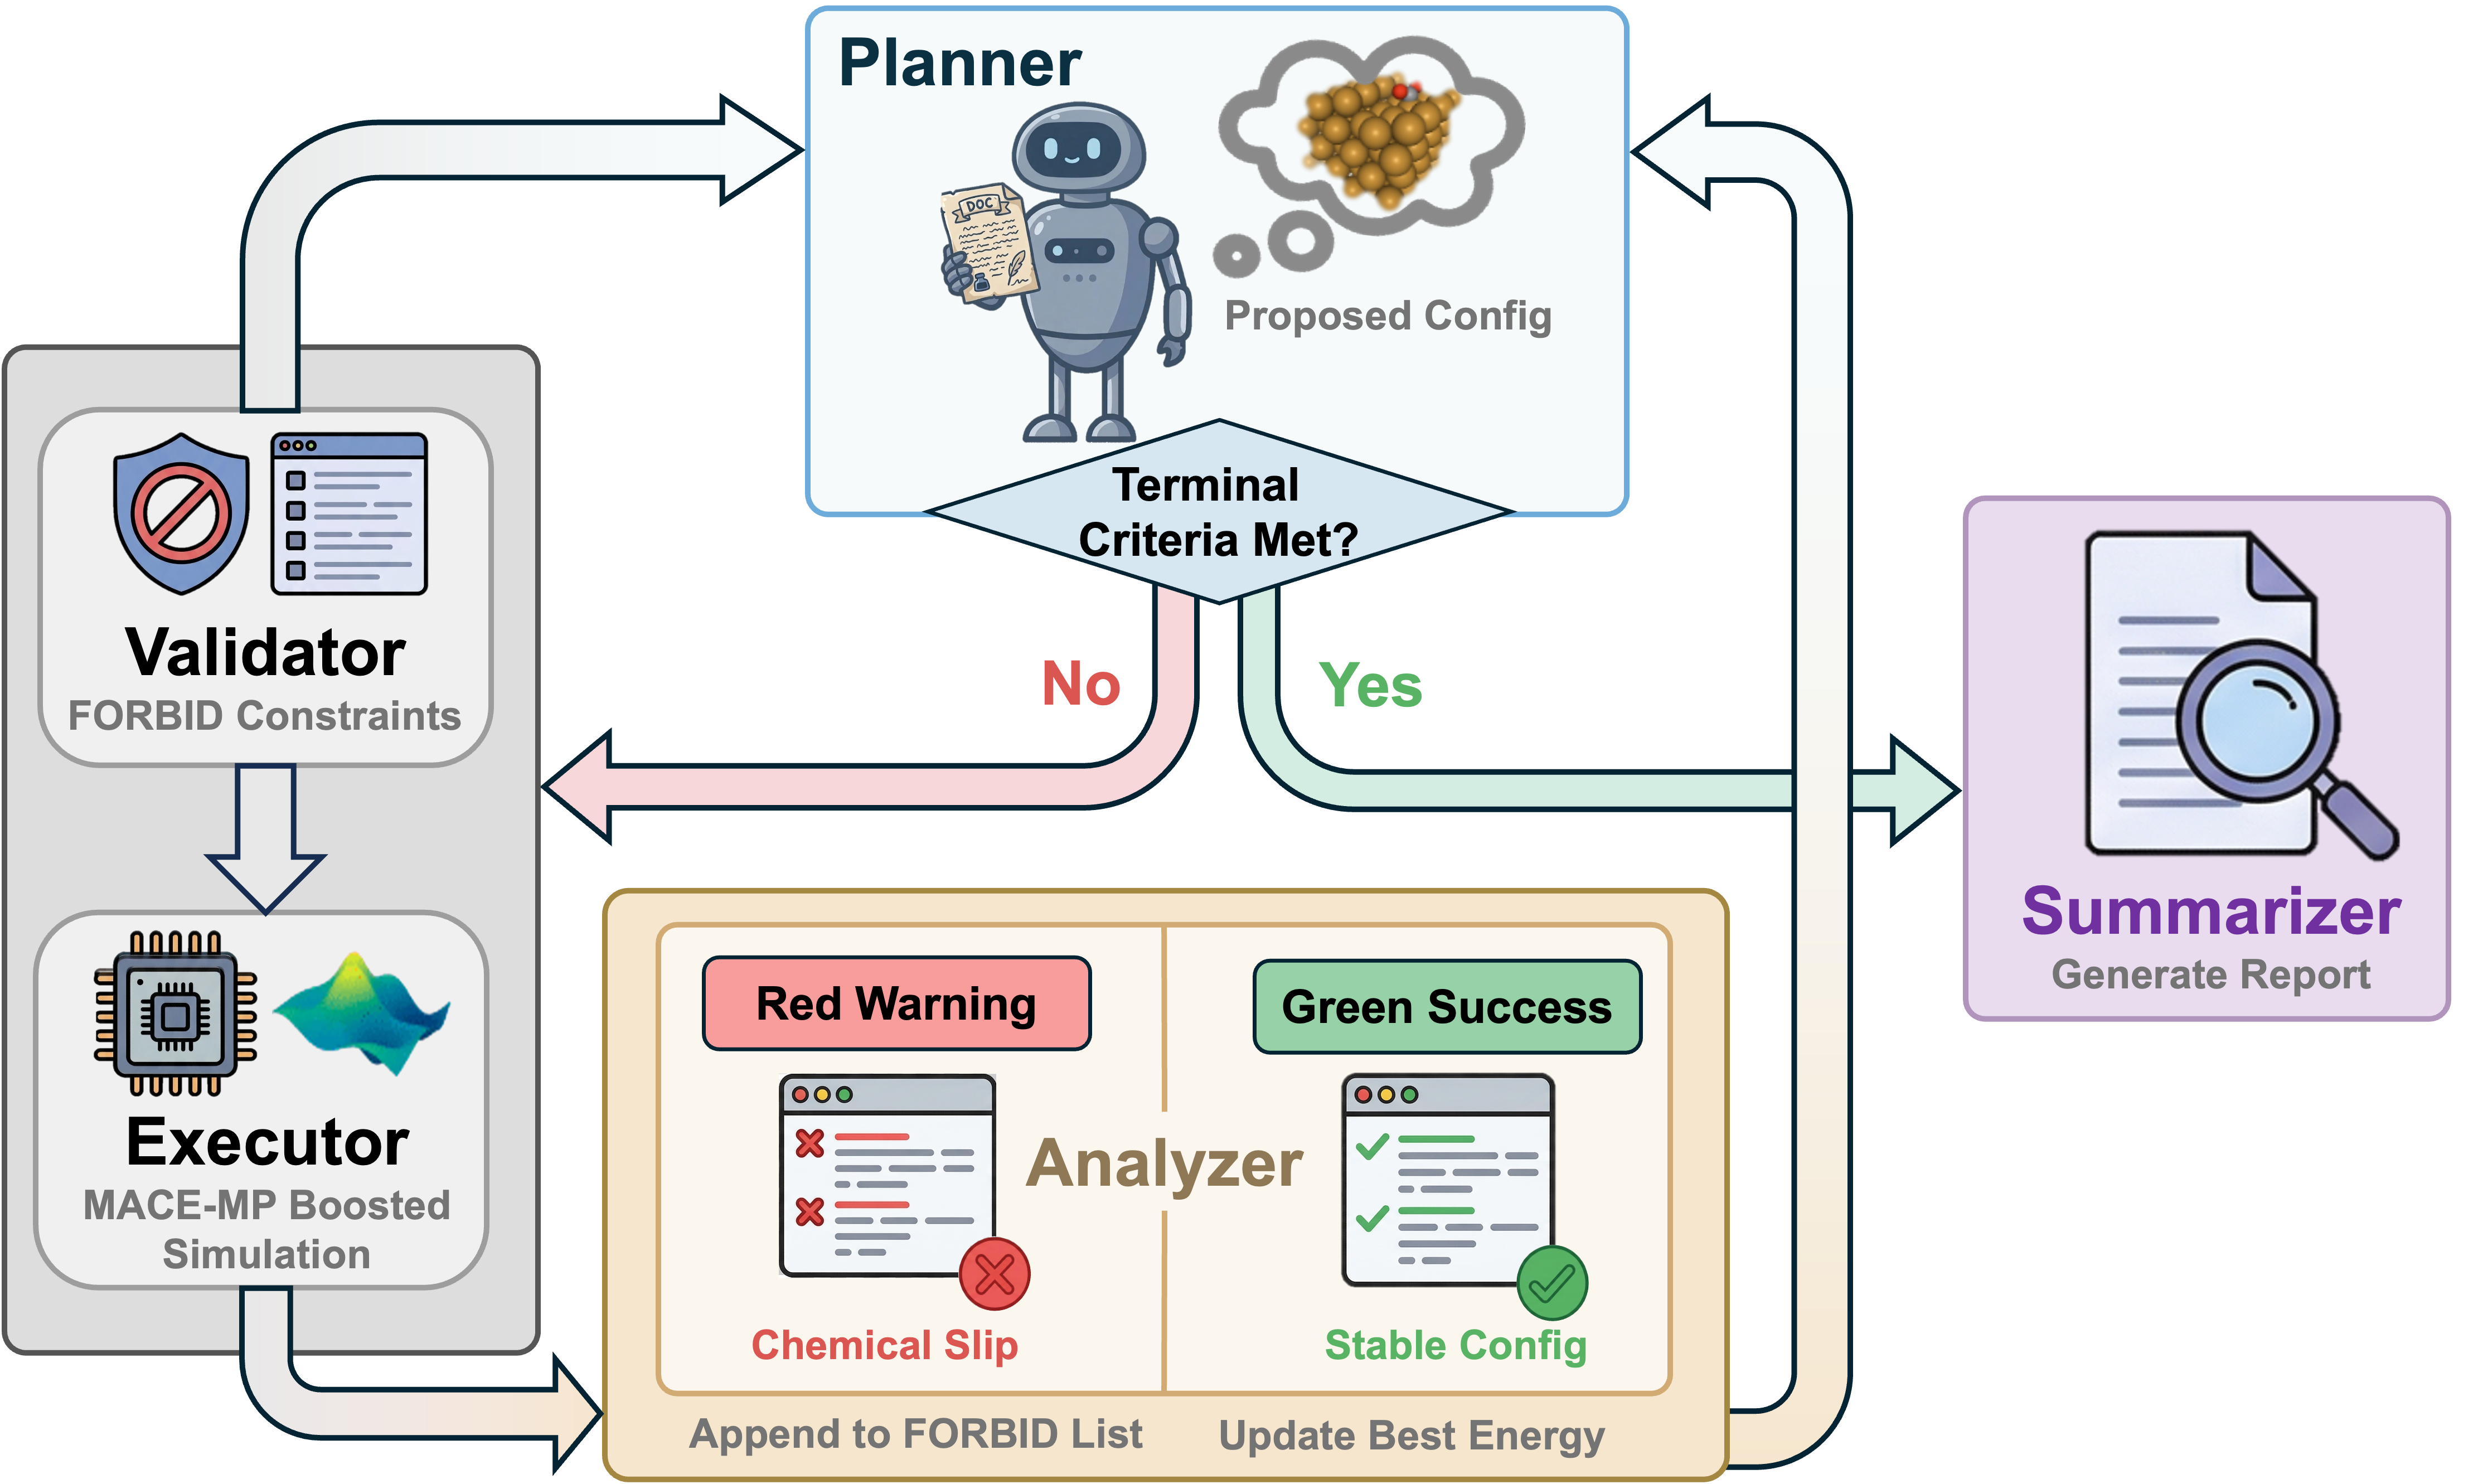
\includegraphics[width=0.75\linewidth]{images/pipeline.png}
    \caption{\textbf{Overview of AdsMind} a. Schematic diagram of AdsMind including the five agents: Planner xxxx Validator xxxx Executor xxxx Analyzer xxxx Summarizer xxxx b. The test benchmark datasets: xxxxx c. Real-world applications comparing with DFT calculations }
    \label{fig:placeholder}
\end{figure}

